\section{Ôn tập chương 1}
\subsection{Đề 1}
\Opensolutionfile{ans}[ans/ans-2-OTC1]
\caulc
%%1
\begin{ex}%[2D1N1-1]
	Hàm số $y=-x^3+3x^2-1$ đồng biến trên khoảng
	\choice
	{$(-\infty;0)$ và $(2;+\infty)$}
	{$(0;3)$}
	{\True $(0;2)$}
	{$(1;+\infty)$}
	\loigiai{
		Tập xác định của hàm số là  $\mathscr{D}=\mathbb{R}$.\\
		Ta có $y'=-3x^2+6x$.\\
		Cho	$y'=0\Leftrightarrow -3x^2+6x=0\Leftrightarrow \hoac {&x=0\\ &x=2.}$\\
		Bảng biến thiên.
		\begin{center}
			
\begin{tikzpicture}
			\tkzTabInit[lgt=1.2,espcl=3]
			{$x$  /1.2, $y'$ /1.2,$y$  /2.5}
			{$-\infty$ , $0$,$2$, $+\infty$}
			\tkzTabLine{,-,z,+,z,-,}
			\tkzTabVar{+/$+\infty$ ,-/$-1$, +/$3$,-/$-\infty$}
			\end{tikzpicture}
		\end{center}
		Dựa vào đồ thị ta có hàm số đồng biến trên $(0;2)$.
	}
\end{ex}
%2
\begin{ex}%[2D1N4-1]
	Đường tiệm cận ngang của đồ thị hàm số $y=\dfrac{2x-4}{x+2}$ là
	\choice
	{\True $y=2$}
	{ $x=2$}
	{$x=-2$}
	{$y=-2$}
	\loigiai{$\underset{x\to -\infty }{\mathop{\lim }}\,\dfrac{2x-4}{x+2}=2$ và $\underset{x\to +\infty }{\mathop{\lim }}\,\dfrac{2x-4}{x+2}=2$ nên hàm số có tiệm cận ngang là $y=2$.
	}
\end{ex} 
%3
\begin{ex}%[2D1N2-2]
	Cho hàm số $y=f(x)$ có bảng biến thiên như sau. 
	\begin{center}
		
\begin{tikzpicture}
		\tkzTabInit[lgt=1.2,espcl=1.5]
		{$x$ /.6,$y'$ /.6,$y$ /1.6}
		{$-\infty$,$-1$,$2$,$+\infty$}
		\tkzTabLine{,+,$0$,-,$0$,+,}
		\tkzTabVar{-/ $-\infty$ ,+/$4$,-/$3$,+/$+\infty$}
		\end{tikzpicture}
	\end{center}
	Giá trị cực tiểu của hàm số bằng
	\choice
	{$4$}
	{$2$}
	{$-1$}
	{\True $3$}
	
	\loigiai{Dựa vào bảng biến thiên, hàm số đạt cực tiểu tại $x=2$. Giá trị cực tiểu là $y_{\text{CT}}=3$.}
\end{ex}
\begin{ex}%[2D1N5-1]
	\immini{
		Đường cong trong hình vẽ bên là đồ thị của hàm số nào dưới đây?
		\choice
		{$y=-x^3-3x^2+2$}
		{\True $y=-x^3+3x^2-2$}
		{$y=x^4-x^2-2$}
		{$y=-x^4+x^2-2$}		
	}
	{
		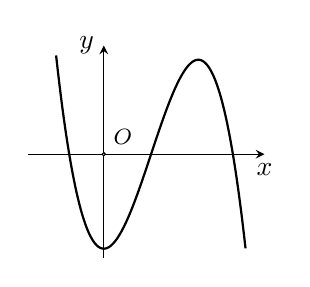
\begin{tikzpicture}[>=stealth,x=1cm,y=1cm,scale=.6]
		\draw[->] (-1.6,0) -- (3.4,0) node[below]{$x$};
		\draw[->] (0,-2.2) -- (0,2.3) node[left]{$y$};
		\draw[thick,smooth,samples=100,domain=-1.01:3.] plot(\x,{-(\x)^3+3*(\x)^2-2});
		\draw [fill=white,draw=black] (0,0) circle (1pt)node[above right]{\footnotesize $O$};
		\end{tikzpicture}
	}
	\loigiai{
		Hàm bậc $3$ và hệ số $ a<0 $ và hệ số $d<0$.
	}
\end{ex}
%4
\begin{ex}%[2D1H2-3]
	Tìm các giá trị $m$ để hàm số $y=x^3-mx-2$ đạt cực đại tại $x=-2$.
	\choice
	{$4$}
	{\True $12$}
	{$-4$}
	{$-12$}
	\loigiai
	{Ta có $y'=3x^2-m$ và $y''=6x$.\\
		Điều kiện cần để hàm số đạt cực đại tại $x=-2$ là
		$$y'(-2)=0\Leftrightarrow 3\cdot (-2)^2-m=0\Leftrightarrow m=12.$$
		Với $m=12$ thì $y''(-2)=-12<0$. Như thế hàm số đạt cực đại tại $x=-2$.\\
		Vậy giá trị $m$ cần tìm là $m=12$.
	}
\end{ex}
%6-11
\begin{ex}%[2D1H2-2]
	\immini{
		Cho hàm số $f(x)$ có đạo hàm $f'(x)$ xác định trên $\mathbb{R}$. Hàm số $y=f'(x)$ có đồ thị như hình bên. Hỏi hàm số $y=f(x)$ có bao nhiêu điểm cực trị?
		\choice
		{$2$}
		{$3$}
		{$4$}
		{\True $1$}
	}{\vspace{-0.4cm}
		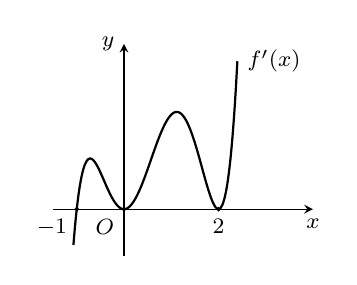
\begin{tikzpicture}[scale=0.6,>=stealth,font=\footnotesize]
		\draw[->] (-1.5,0)--(4,0) node[below] {$x$};
		\draw[->] (0,-1)--(0,3.5) node[left] {$y$};
		\draw[smooth,samples=100,thick,domain=-1.07:2.4] plot(\x,{(\x+1)*(\x)^2*(\x-2)^2}) node[right]{$f'(x)$};
		\filldraw (-1,0) circle (1pt) node[below left] {$-1$};
		\filldraw (2,0) circle (1pt) node[below] {$2$};
		\filldraw (0,0) circle (1pt) node[below left] {$O$};
		\end{tikzpicture}
	}
	\loigiai{
		Dựa vào đồ thị ta thấy $f'(-1)=0$ và $f'(x)<0,\ \forall x<-1$ và $f'(x)\geq 0,\ \forall x>-1$.\\
		Suy ra $x=-1$ là điểm cực trị duy nhất của đồ thị.
	}
\end{ex}
%7

%8
\begin{ex}%[2D1H2-1]
	Cho hàm số $f$ có đạo hàm $f'(x)=(x+1)^2(x-2)^3(2x+3)$. Tìm số điểm cực trị của hàm số $f$.
	\choice
	{ $ 3 $}
	{ \True $ 2 $}
	{ $ 1 $}
	{ $ 0 $}
	\loigiai{
		Ta có $$f'(x)=0 \Leftrightarrow \hoac{& x=-1~\text{(kép)}\\& x=2~\text{(bội lẻ)}\\& x=-\dfrac{3}{2}~\text{(đơn).}}$$\\
		Vì $f'(x)$ đổi dấu khi $x$ qua nghiệm đơn hoặc bội lẻ nên hàm số $f$ có $2$ cực trị.
	}
\end{ex}
%9
\begin{ex}
	Đồ thị hàm số $y= \dfrac{2x-1}{x- 1}$ cắt đường thẳng $y= x- 1$ tại mấy điểm phân biệt?
	\choice
	{\True $2$}
	{$1$}
	{$3$}
	{$0$}
	\loigiai{
		Điều kiện $x \ne 1$.\\
		Ta xét phương trình hoành độ giao điểm\\
		$\dfrac{2x- 1}{x- 1}= x- 1 \Leftrightarrow 2x- 1= x^2- 2x+ 1 \Leftrightarrow x^2- 4x+ 2= 0 \Leftrightarrow \hoac{&x= 2+ \sqrt{2}\\&x= 2- \sqrt{2}\ \text{(thỏa mãn)}.}$\\
		Vậy đồ thị hàm số $y= \dfrac{2x-1}{x- 1}$ cắt đường thẳng $y= x- 1$ tại hai điểm phân biệt.
	}
\end{ex}
%9
\begin{ex}%[2D1H1-1]
	Hàm số nào dưới đây đồng biến trên $\mathbb{R}$?
	\choice
	{$y=x^4-x^2$}
	{$y=x^3-x$}
	{$y=\dfrac{x-1}{x+2}$}
	{\True $y=x^3+x$}
	\loigiai{
		Xét hàm số $y=x^3+x$ có tập xác định $\mathscr{D}=\mathbb{R}$.\\
		Ta có $y'=3x^2+1$ nên $y'>0,\, \forall x \in \mathbb{R}$.\\
		Vậy hàm số $y=x^3+x$ đồng biến trên $\mathbb{R}$.
	}	
\end{ex}
%10
\begin{ex}%[2D1H5-4]
	\immini{Cho hàm số $y=f(x)$ liên tục trên $\mathbb {R}$ và có đồ thị như hình bên. Phương trình $f(x)=\pi$ có bao nhiêu nghiệm thực phân biệt?
		\choice
		{$3$}
		{\True $4$}
		{$2$}
		{$1$}
	}{\vspace{-0.8cm}
		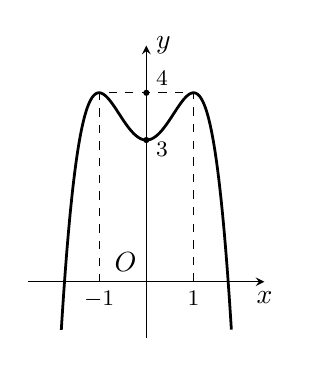
\begin{tikzpicture}[smooth,samples=300,scale=0.6,>=stealth]
		\draw[->] (-2.5,0)--(2.5,0) node[below]{$x$};
		\draw[->] (0,-1.2)--(0,5) node[right]{$y$};
		\draw (0,0) node[above left]{$O$};
		\draw[smooth,line width = 1pt,domain=-1.8:1.8] plot(\x,{-(\x)^4 + 2*(\x)^2+3});
		\draw[fill=black] (0,3) circle(1.5pt) (0,4) circle(1.5pt);
		\draw[dashed] (1,0)node[below]{\footnotesize$1$}--(1,4)--(-1,4)--(-1,0)node[below]{\footnotesize$-1$};
		\node[right] at (0,2.8){\footnotesize $3$};
		\node[right] at (0,4.3){\footnotesize $4$};
		\end{tikzpicture}}
	\loigiai{
		Số nghiệm của phương trình $f(x )=\pi $ bằng số giao điểm của đường thẳng $y=\pi $ và đồ thị hàm số $y=f\left(x \right) $.\\
		Dựa vào đồ thị ta thấy đường thẳng $y=\pi $ cắt đồ thị tại $4$ điểm phân biệt nên phương trình có $4$ nghiệm phân biệt.
	}
\end{ex}
%11

%12
\begin{ex}%[2D1V2-4]
	Có bao nhiêu giá trị nguyên của tham số $m$ sao cho ứng với mỗi $m$, hàm số $y=-x^3+3 x^2-3 m x+\dfrac{5}{3}$ có đúng một điểm cực trị thuộc khoảng $(-2 ; 5)$?
	\choice
	{$16$}
	{$6$}
	{$17$}
	{\True $7$}
	\loigiai{
		Ta có $y' = -3x^2+6x-3 m$; $y'= 0 \Leftrightarrow m= -x^2+2x$. \quad (1)\\
		Xét hàm số $g(x) = -x^2+2x$ trên khoảng $(-2 ; 5)$.  \\
		Bảng biến thiên của hàm số $g(x)$ 
		\begin{center}
			
\begin{tikzpicture}
			\tkzTabInit[nocadre=false,lgt=1.2,espcl=2.5,deltacl=0.6]
			{$x$ /0.7,$g'(x)$ /0.7,$g(x)$ /2}
			{$-2$,$1$,$5$}
			\tkzTabLine{,+,$0$,-,}
			\tkzTabVar{-/$-8$,+/$1$,-/$-15$ }
			\end{tikzpicture}
		\end{center}
		Từ bảng biến thiên suy ra hàm số đã cho có đúng một điểm cực trị thuộc khoảng $(-2 ; 5)$ khi và chỉ khi phương trình (1) có đúng một nghiệm bội lẻ thuộc $(-2 ; 5)$, suy ra  $-15 < m \leq -8$. \\
		Mặt khác,  $m$ nguyên suy ra $m \in \{ -14;-13;\ldots;-8\}$. \\
		Vậy có tất cả $7$ giá trị nguyên của tham số $m$ thỏa mãn.
	}
\end{ex}
%12
\begin{ex}%[2D1V4-2]
	Cho hàm số $y=\dfrac{x+1}{x^2-2mx+4}$. Tìm tất cả các giá trị của tham số $m$ để đồ thị có ba đường tiệm cận.
	\choice
	{\True$\hoac{&	m<-2\\ & m>2}$ và $m\neq -\dfrac{5}{2}$}
	{$m>2$}
	{$\heva{& m<-2 \\ & m\neq -\dfrac{5}{2}}$}
	{$\hoac{&	m<-2\\ & m>2}$}
	\loigiai{
		Đồ thị hàm số luôn có $1$ tiệm cận ngang $y=0$ nên để có ba đường tiệm cận thì đồ thị có hai đường tiệm cận đứng, hay $x^2-2mx+4=0$ có nghiệm khác $-1$\\
		$$\Leftrightarrow \heva{& m^2-4>0 \\ & (-1)^2-2m(-1) +4 \neq 0} \Leftrightarrow \heva{ & m<-2~\text{hoặc}~m>2\\ & m\neq -\dfrac{5}{2}.}$$
	}
\end{ex}

\Closesolutionfile{ans}
\indapan{6}{ans/ans-2-OTC1}

\cauds
\Opensolutionfile{ans}[ans/ans-2-OTC1-DS]
%%%%1
\begin{ex}%[2D1V4-3]
	Cho hàm số $ y = \dfrac{{{x^2} + 2x - 2}}{{x - 1}} $. 
	Các phát biểu sau đây đúng hay sai?
	\choiceTF
	{\True Tập xác định của hàm số là $\mathscr{D} = \mathbb{R} \setminus \left\{ 1 \right\}$}
	{\True $y' = 0 \Leftrightarrow x = 0$  hoặc $x = 2$}
	{Đường thẳng $y = x$  là tiệm cận xiên của đồ thị hàm số}
	{Số giá trị nguyên của tham số $m$ để phương trình $\left|f(x) \right|-m=0 $ có $4$ nghiệm bé hơn $1$ là $3$}
	\loigiai{
		\begin{itemchoice}
			\itemch Đúng. Vì tập xác định của hàm số là $\mathscr{D} = \mathbb{R} \setminus \left\{ 1 \right\}$.
			\itemch Đúng. Vì đạo hàm $y' = \dfrac{{{x^2} - 2x}}{{{{(x - 1)}^2}}}$.\\
			Suy ra $y' = 0 \Leftrightarrow x = 0$  hoặc $x = 2$.
			\itemch Sai.Vì\\
			$a = \mathop {{\rm{lim}}}\limits_{x \to  + \infty } \dfrac{{{x^2} + 2x - 2}}{x(x -1)} = 1$ và $b = \mathop {{\rm{lim}}}\limits_{x \to  + \infty } \left( {\dfrac{{{x^2} + 2x - 2}}{{x - 1}} - x} \right) = \mathop {{\rm{lim}}}\limits_{x \to  + \infty } \dfrac{{3x - 2}}{{x - 1}} = 3$.\\ 
			Suy ra đường thẳng $y = x + 3$  là tiệm cận xiên của đồ thị hàm số.
			\itemch Sai. Vì hàm số $y=\left| f(x)\right| $ có bảng biên thiên là
			\begin{center}
				\begin{tikzpicture}[scale=1, font=\footnotesize, line join=round, line cap=round, >=stealth]
				\tkzTabInit[nocadre=false,lgt=1.2,espcl=2.2,deltacl=0.6]
				{$x$ /0.6,$y'$ /0.6,$y$ /1.6}
				{$-\infty$,$0$,$1$,$2$,$+\infty$}
				\tkzTabLine{,+,0,-,d,-,0,+,}
				\tkzTabVar{-/$-\infty$,+/$2$,-D+/$-\infty$/$+\infty$,-/$6$,+/$+\infty$}
				\draw[red, dashed, name path=a] ($(N12)!0.5!(N13)$)-- ($(N32)!0.5!(N33)$);
				\path[name path=b] (N13)--(N22);
				\path[name path=c] (N22)--(N33);
				\path [name intersections={of=a and b,by=A}];
				\path [name intersections={of=a and c,by=B}];
				\draw[->, red, thick] ($(N12)+(0,-0.4)$)node[above]{$+\infty$}--(A)node[below]{$0$};
				\draw[->,red,thick] ($(B)+(-0.23,0)$)node[below]{$0$}--($(N32)+(-0.4,-0.4)$)node[above]{$+\infty$};
				\end{tikzpicture}
			\end{center}
			Dựa vào bảng biến thiên, ta suy ra phương trình đã cho có $4$ nghiệm nhỏ hơn $1$ khi $0<m<2$.\\
			Vì $m$ là số nguyên nên $m=1$.	
		\end{itemchoice}
	}
\end{ex}
%%%%2
\begin{ex}%[2D1V5-1]
	\immini{Cho hàm số $y=f(x)=\dfrac{ax^2+bx+c}{x+b'}$ (với $a$, $b$, $c$, $b'$ là các số thực) có đồ thị như hình bên. Xét tính đúng hay sai của các khẳng định sau
		\choiceTF
		{\True $ x=0 $ là một đường tiệm cận đứng của đồ thị hàm số}
		{Hàm số đã cho có một điểm cực trị}
		{\True $ y=x $ là một đường tiệm cận xiên của đồ thị hàm số}
		{Các hệ số $a$, $b$, $c$, $b'$ có tất cả là $3$ số dương }
	}{
		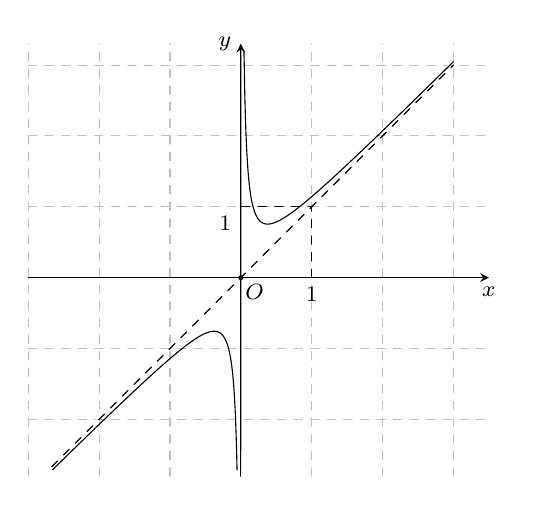
\begin{tikzpicture}[scale=.9, font=\footnotesize, line join=round, line cap=round,>=stealth]
		\def\a{0} \def\b{1} \def\c{1} \def\d{-1} % Hệ số
		\def\xmin{-3} \def\xmax{3.5}
		\def\ymin{-2.8} \def\ymax{3.3} 
		\draw[color=gray!50,dashed] (\xmin,\ymin) grid (\xmax,\ymax); 
		\draw[->] (\xmin,0)--(\xmax,0) node [below]{$x$};
		\draw[->] (0,\ymin)--(0,\ymax) node [left]{$y$};
		\draw[dashed] (1,0)node [below]{$1$}--(1,1)--(0,1)node [below left]{$1$};
		\fill (0,0) circle(1pt) node[shift=(-45:0.25)]{$O$}; 
		\clip (\xmin+0.1,\ymin+0.1) rectangle (\xmax-0.1,\ymax-0.1);
		\draw[smooth,samples=300,domain=-3:3] plot(\x,{\x+1/(7*\x)});
		\draw[dashed,smooth,samples=300,domain=-3:3] plot(\x,{\x});
		
		\end{tikzpicture}}
	
	\loigiai{
		\begin{itemchoice}
			\itemch Đúng. Vì $ x=0 $ là một đường tiệm cận đứng của đồ thị hàm số.
			\itemch Sai. Vì	hàm số đã cho có hai điểm cực trị.
			\itemch Đúng. Vì $ y=x $ là một đường tiệm cận xiên của đồ thị hàm số.
			\itemch Sai. Vì từ đồ thị hàm số $y=f(x)$ ta suy ra $f(x)=x+\dfrac{c}{x}$.\\
			Do đó, tiệm cận đứng $x=0$ suy ra $b'=0$.\\
			Từ đó suy ra $f(x)=x+b+\dfrac{c}{x}$ nên $b=0$ và $a=1>0$.\\
			Do đồ thị hàm số có $2$ cực trị nên phương trình $f'(x)=0$ có $2$ nghiệm phân biệt. Hay phương trình $\dfrac{x^2-c}{x^2}=0$ có $2$ nghiệm phân biệt, suy ra $c>0$.\\
			Vậy, có hai hệ số dương.
		\end{itemchoice}	
	}
\end{ex}
%%%%3
\begin{ex}%[2D1H5-4]
	\immini{Cho hàm số bậc ba $y=f(x)$ có đồ thị như hình vẽ bên. Mỗi mệnh đề sau đây đúng hay sai?
		\choiceTF
		{\True Phương trình $f(x)=0$ có $2$ nghiệm}
		{Phương trình $f(x)=1$ vô nghiệm}
		{Phương trình $f(x)+1=0$ có $2$ nghiệm}
		{\True Phương trình $f(x)=x$ có $3$ nghiệm}}
	{
		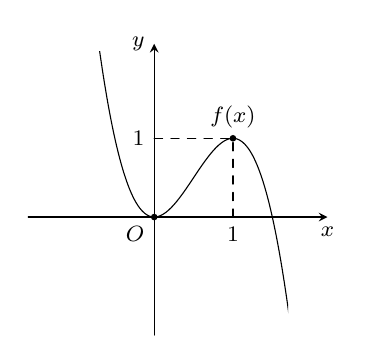
\begin{tikzpicture}[scale=1,>=stealth, font=\footnotesize, line join=round, line cap=round]
		\def\a{-2} \def\b{3} \def\c{0} \def\d{0} % Hệ số
		\def\xmin{-1.6} \def\xmax{2.2}
		\def\ymin{-1.5} \def\ymax{2.2}
		\draw[->] (\xmin,0)--(\xmax,0) node [below]{$x$};
		\draw[->] (0,\ymin)--(0,\ymax) node [left]{$y$};
		\node at (0,0) [below left]{$O$};
		\clip (\xmin+0.1,\ymin+0.1) rectangle (\xmax-0.5,\ymax-0.1);
	\draw (1,1) node[above]{$f(x)$};
		\draw[smooth,samples=300] plot(\x,{\a*(\x)^3+\b*(\x)^2+\c*(\x)+\d});
		\draw[dashed] (0,1)node[left]{$1$}-|(1,0)node[below]{$1$};
		\foreach \x/\y in{0/0,1/1} \fill (\x,\y) circle(1.2pt);
		\end{tikzpicture}
	}
	\loigiai{
		\begin{itemchoice}
			\itemch  
			\immini{Đúng. Vì từ đồ thị của hai hàm số $y=f(x)$ và $y=0$ như hình vẽ\\
				Dựa vào hình vẽ, ta có phương trình $f(x)=0$ có $2$ nghiệm phân biệt.}
			{
				\begin{tikzpicture}[scale=1,>=stealth, font=\footnotesize, line join=round, line cap=round]
				\def\a{-2} \def\b{3} \def\c{0} \def\d{0} % Hệ số
				\def\xmin{-1.6} \def\xmax{2.2}
				\def\ymin{-1.5} \def\ymax{2.2}
				\draw[->] (\xmin,0)--(\xmax,0) node [below]{$x$};
				\draw[->] (0,\ymin)--(0,\ymax) node [left]{$y$};
				\node at (0,0) [below right]{$O$};
				\clip (\xmin+0.1,\ymin+0.1) rectangle (\xmax-0.5,\ymax-0.1);
				\draw[smooth,samples=300] plot(\x,{\a*(\x)^3+\b*(\x)^2+\c*(\x)+\d});
				\draw[smooth,samples=300] plot(\x,{(0)});
				\draw[dashed] (0,1)node[left]{$1$}-|(1,0)node[below]{$1$};
				\foreach \x/\y in{0/0,1/1} \fill (\x,\y) circle(1.2pt);
				\end{tikzpicture}
			}
			\itemch 
			\immini{Sai. Vì từ đồ thị của hai hàm số $y=f(x)$ và $y=1$ như hình vẽ\\
				Dựa vào hình vẽ, ta có phương trình $f(x)=1$ có $2$ nghiệm phân biệt.}
			{
				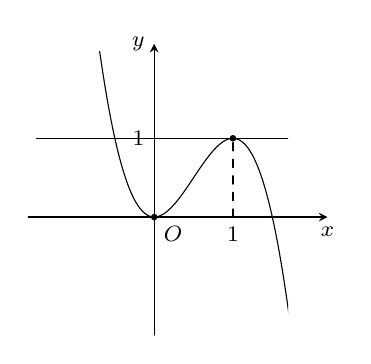
\begin{tikzpicture}[scale=1,>=stealth, font=\footnotesize, line join=round, line cap=round]
				\def\a{-2} \def\b{3} \def\c{0} \def\d{0} % Hệ số
				\def\xmin{-1.6} \def\xmax{2.2}
				\def\ymin{-1.5} \def\ymax{2.2}
				\draw[->] (\xmin,0)--(\xmax,0) node [below]{$x$};
				\draw[->] (0,\ymin)--(0,\ymax) node [left]{$y$};
				\node at (0,0) [below right]{$O$};
				\clip (\xmin+0.1,\ymin+0.1) rectangle (\xmax-0.5,\ymax-0.1);
				\draw[smooth,samples=300] plot(\x,{\a*(\x)^3+\b*(\x)^2+\c*(\x)+\d});
				\draw[smooth,samples=300] plot(\x,{(1)});
				\draw[dashed] (0,1)node[left]{$1$}-|(1,0)node[below]{$1$};
				\foreach \x/\y in{0/0,1/1} \fill (\x,\y) circle(1.2pt);
				\end{tikzpicture}
			}
			\itemch 
			\immini{Sai. Vì từ đồ thị của hai hàm số $y=f(x)$ và $y=-1$ như hình vẽ\\
				Dựa vào hình vẽ, ta có phương trình $f(x)=-1$ có $1$ nghiệm duy nhất.}
			{
				\begin{tikzpicture}[scale=1,>=stealth, font=\footnotesize, line join=round, line cap=round]
				\def\a{-2} \def\b{3} \def\c{0} \def\d{0} % Hệ số
				\def\xmin{-1.6} \def\xmax{3.2}
				\def\ymin{-1.5} \def\ymax{2.2}
				\draw[->] (\xmin,0)--(\xmax,0) node [below]{$x$};
				\draw[->] (0,\ymin)--(0,\ymax) node [left]{$y$};
				\node at (0,0) [below right]{$O$};
				\clip (\xmin+0.1,\ymin+0.1) rectangle (\xmax-0.5,\ymax-0.1);
				\draw[smooth,samples=300] plot(\x,{\a*(\x)^3+\b*(\x)^2+\c*(\x)+\d});
				\draw[smooth,samples=300] plot(\x,{(-1)});
				\draw[dashed] (0,1)node[left]{$1$}-|(1,0)node[below]{$1$};
				\foreach \x/\y in{0/0,1/1} \fill (\x,\y) circle(1.2pt);
				\end{tikzpicture}
			}
			\itemch 
			\immini{Đúng. Vì từ đồ thị của hai hàm số $y=f(x)$ và $y=x$ như hình vẽ\\
				Dựa vào hình vẽ, ta có phương trình $f(x)=x$ có $3$ nghiệm phân biệt.}
			{
				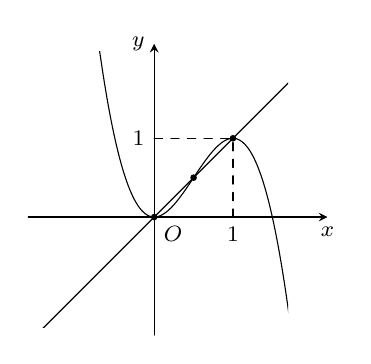
\begin{tikzpicture}[scale=1,>=stealth, font=\footnotesize, line join=round, line cap=round]
				\def\a{-2} \def\b{3} \def\c{0} \def\d{0} % Hệ số
				\def\xmin{-1.6} \def\xmax{2.2}
				\def\ymin{-1.5} \def\ymax{2.2}
				\draw[->] (\xmin,0)--(\xmax,0) node [below]{$x$};
				\draw[->] (0,\ymin)--(0,\ymax) node [left]{$y$};
				\node at (0,0) [below right]{$O$};
				\clip (\xmin+0.1,\ymin+0.1) rectangle (\xmax-0.5,\ymax-0.1);
				\draw[smooth,samples=300] plot(\x,{\a*(\x)^3+\b*(\x)^2+\c*(\x)+\d});
				\draw[smooth,samples=300] plot(\x,{(\x)});
				\draw[dashed] (0,1)node[left]{$1$}-|(1,0)node[below]{$1$};
				\foreach \x/\y in{0/0,1/1,0.5/0.5} \fill (\x,\y) circle(1.2pt);
				\end{tikzpicture}
			}
		\end{itemchoice}
	}
\end{ex}
\begin{ex}%[2D1H4-1]
	Cho hàm số hàm số $y=\dfrac{-4x+5}{2x+3}$ có đồ thị $(C)$.
	Xét tính đúng hoặc sai của các khẳng định sau
	\choiceTF
	{\True Hàm số không có cực trị}
	{Đồ thị hàm số có tiệm cận đứng $x=-3$}
	{\True Đồ thị hàm số có tiệm cận ngang $y=-2$}
	{\True Các đường tiệm cận của đồ thị tạo với hai trục toạ độ một hình chữ nhật có diện tích bằng $3$}
	\loigiai{
		\begin{itemchoice}
			\itemch Đúng. Vì $y'=\dfrac{-22}{(2x+3)^2}<0,\, \forall x \ne \dfrac{-3}{2}$ nên hàm số không có cực trị.
			\itemch Sai. Vì  tập xác định $\mathscr D=\mathbb{R}\setminus \left \{-\dfrac{3}{2}\right \}$.\\
			$\lim \limits_{x\to \left (-\frac{3}{2}\right )^+}y=+\infty; \ \lim \limits_{x\to \left (-\frac{3}{2}\right )^-}y=-\infty$ nên đồ thị hàm số có tiệm cận đứng $x=-\dfrac{3}{2}$.
			\itemch Đúng. Vì $$\lim \limits_{x\to -\infty}y=-2,\,\lim \limits_{x\to +\infty}y=-2$$ nên đồ thị hàm số có một tiệm cận ngang là $y=-2$.
			\itemch Đúng. Vì diện tích hình chữ nhật cần tìm là $S=\left |-\dfrac{3}{2}\right |\cdot \left |-2\right |=3$.
		\end{itemchoice}	
		
	}
\end{ex}


\Closesolutionfile{ans}
\indapan{3}{ans/ans-2-OTC1-DS}


\Opensolutionfile{ans}[ans/ans-2-OTC1-TLN]
\caukq
\begin{ex}%[2D1H5-4]
	\immini{Cho hàm số bậc bốn $y=f(x)$ có đồ thị là đường cong trong hình bên. Có bao nhiêu giá trị nguyên của tham số $m$ sao cho ứng với mỗi $m$, phương trình $2f(x)=m$ có $4$ nghiệm thực phân biệt?}
	{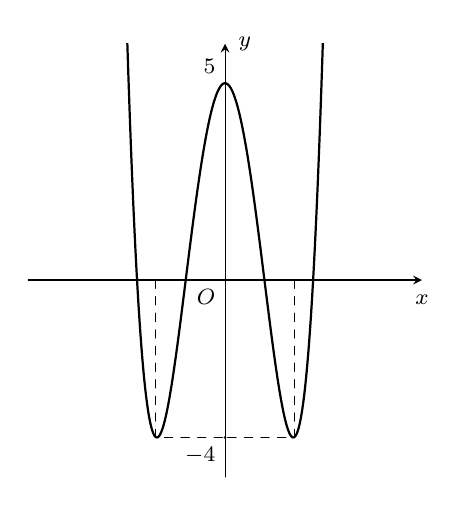
\begin{tikzpicture}[scale=.5,>=stealth, font=\footnotesize, line join=round, line cap=round]	
		\tikzset{label style/.style={font=\footnotesize}}
		\def \xmin{-5}\def \xmax{5}\def \ymin{-5}\def \ymax{6} 
		\draw[->] (\xmin,0)--(\xmax,0) node[shift=(-90:0.25)] {$x$};
		\draw[->] (0,\ymin)--(0,\ymax) node[shift=(0:0.25)] {$y$};
		\fill[black] 
		(0,0)node [below left]{$O$} circle(1pt) 
		(0,5)node [above left]{$5$} circle(1pt)
		(0,-4)node [below left]{$-4$} circle(1pt)
		; 
		\draw[dashed] (-1.76,0)|-(0,-4) (1.76,0)|-(0,-4);
		\begin{scope}
		\clip (\xmin,\ymin) rectangle (\xmax,\ymax); 
		\draw[thick,samples=300,domain=\xmin:\xmax,smooth,variable=\x] plot
		(\x,{1*((\x)^4)-6*((\x)^2)+5});
		\end{scope}
		\end{tikzpicture}}
		\shortans{$17$}
	\loigiai{
		Xét phương trình $$2f(x)=m\Leftrightarrow f(x)=\dfrac{m}{2}$$
		có $4$ nghiệm thực phân biệt khi và chỉ khi 
		$$-4<\dfrac{m}{2}<5\Leftrightarrow -8<m<10.$$
		Vì $m\in \mathbb{Z}$ nên $m\in \{-7;-6;\ldots;8;9\}$ nên có $17$ giá trị nguyên của $m$ thỏa yêu cầu bài toán.
	}
\end{ex}
\begin{ex}%[2D1V4-3]
	Hàm số $y=\dfrac{x^2+2x+3}{x+1}$ có tâm đối xứng là $I(a;b)$. Giá trị $2a+b$ bằng bao nhiêu?
\shortans{$-1$}
\loigiai{
Ta có  $y=\dfrac{x^2+2x+3}{x+1}=x+1+\dfrac{2}{x+1}$ nên đồ thị hàm số có phương trình đường tiệm cận xiên và tiệm cận đứng lần lượt là $y=x+1$ và $x=-1$.\\
Tâm đối xứng của đồ thị là giao điểm của hai đường tiệm cận nên thỏa hệ $$\heva{ &  y=x+1\\&x=-1 } \Leftrightarrow \heva{ &x=-1\\&y=0.}$$
Suy ra $I(-1;0)$ hay $2a+b=-1.$
}
\end{ex}
\begin{ex}%[2D1V1-3]
	Cho hàm số $y = \dfrac{mx - 2m - 3}{x - m}$ với $m$ là tham số. Gọi $S$ là tập hợp tất cả các giá trị nguyên của $m$ để hàm số đồng biến trên các khoảng xác định. Tìm số phần tử của $S$.
\shortans{$3$}
	\loigiai{
		Xét hàm số $y = \dfrac{mx - 2m - 3}{x - m}$.\\
		Ta có $y' = \dfrac{- m^2 + 2m + 3}{\left(x - m\right)^2}$ hàm số đồng biến trên các khoảng xác định 
		$$\Leftrightarrow y' > 0 \Leftrightarrow - m^2 + 2m + 3 > 0 \Leftrightarrow m \in \left(-1;3\right)\,(m \in \mathbb{Z}) \Rightarrow m \in \left\lbrace 0;1;2\right\rbrace.$$
Vậy tập $S$ có $3$ phần tử nguyên.
	}
\end{ex}

\begin{ex}%[2D1V3-6]
	Một vật chuyển động theo quy luật $s=-\dfrac{1}{3} t^3 + 6 t^2$ với $t$ (giây) là khoảng thời gian tính từ khi vật bắt đầu chuyển động và $s$ (mét) là quãng đường vật di chuyển được trong khoảng thời gian đó. Hỏi trong khoảng thời gian $9$ giây, kể từ khi bắt đầu chuyển động, vận tốc lớn nhất của vật đạt được bằng bao nhiêu m/s?
	\shortans{$36$}
	\loigiai{
		Vận tốc của vật được tính bởi $v(t)=-t^2+12t$.\\
		Ta có $v'(t)=-2t+12$. Cho $v'(t)=0$ ta được $t=6.$\\
		Bảng biến thiên
		\begin{center}
			
\begin{tikzpicture}[font=\footnotesize, line join=round, line cap=round]
			\tkzTabInit[nocadre=false,lgt=1.5,espcl=3]
			{$t$ /0.6, $v'$ /.6,$v$ /2}
			{$0$ ,$6$ ,$9$}
			\tkzTabLine{,+,0,-,}
			\tkzTabVar{ -/$0$,+/$36$,-/$27$}
			\end{tikzpicture}
		\end{center}
		Dựa vào bảng biến thiên ta có vận tốc lớn nhất của vật đạt được bằng $36$ m/s.
	}
\end{ex}
%%%%5VVDC1
\begin{ex}%[2D1C3-6]
	Thể tích $V$ của $1$ kg nước (tính bằng $\text{cm}^3$) ở nhiệt độ $T$ (đơn vị: $^\circ C$) khi $T$ thay đổi từ $^\circ C$ đến $30^\circ C$ được cho xấp xỉ bởi công thức
	$$V=999{,}87-0{,}06426T+0,0085043T^2-0{,}0000769T^3.$$
	(Nguồn: James Stewart, J. (2015). Calculus.Cengage Learning 8th edition, p.284)\\ Tìm nhiệt độ $T_0 \in \left(0;30\right)$ để kể từ nhiệt độ $T_0$ trở lên thì thể tích $V$ tăng (làm tròn kết quả đến hàng đơn vị).
	\shortans{$4$}
	\loigiai{Xét hàm số $f\left(T\right)=V=999{,}87-0{,}06426T+0,0085043T^2-0{,}0000769T^3$.\\ Hàm số xác định trên khoảng $\left(0;30\right)$.\\
		Ta có $f'\left(T\right)=-2{,}307 \cdot 10^{-4}T^2+0{,}0170086T-0{,}06426$.
		$$f'\left(T\right)=0\Leftrightarrow \hoac{&T \approx 3{,}6\\&T\approx -77{,}33}\Leftrightarrow T\approx3{,}6.$$
	Ta có bảng biến thiên sau
		\begin{center}
			
\begin{tikzpicture}[font=\footnotesize, line join=round, line cap=round]
			\tkzTabInit[lgt=1.2,espcl=3]
			{$T$ /.7, $f’(T)$ /.7, $f(T)$ /3}
			{$0$,$3{,}6$,$30$}
			\tkzTabLine{ ,-,z,+,}
		\tkzTabVar{+/$f(0)$,-/$f(3{,}6)$,+/$f(30)$}
			\end{tikzpicture}
		\end{center}
		Vậy $T_0=4^\circ C$ trở lên thì nhiệt độ tăng.
	}
\end{ex}
\begin{ex}%[2D1C2-6]
	Cho hàm số $f(x)$ có đạo hàm $f'(x)=x^2-82 x$. Có bao nhiêu giá trị nguyên dương của tham số $m$ để hàm số $y=f\left(x^4-18 x^2+m\right)$ có đúng $7$ cực trị.
	\shortans{$80$}
		\loigiai{
		Ta có
		\begin{eqnarray*}
			& y'=\left(4 x^3-36 x\right) \cdot f^{\prime}\left(x^4-18 x^2+m\right). \\
			& y'=0 \Leftrightarrow \hoac{& f'\left(x^4-18x^2+m\right)=0\\& 4x^3-36x=0}
		\end{eqnarray*}
		\begin{itemize}
			\item Với $4x^3-36x=0 \Leftrightarrow\hoac{&x=0\\&x=\pm 3}$ có $3$ nghiệm đơn.
			\item $f'\left(x^4-18 x^2+m\right)=0 \Leftrightarrow \hoac{& x^4-18x^2+m=0\\& x^4-18x^2+m=82}\Leftrightarrow\hoac{& x^4-18x^2=-m\\&x^4-18x^2=-m+82.}$\\
			Xét hàm số $g(x)=x^4-18 x^2$ có $g'(x)=0 \Leftrightarrow \hoac{& x=0\\&x=\pm 3.}$\\
			Ta có bảng biến thiên của hàm số $g(x)=x^4-18 x^2$ 
			\begin{center}
				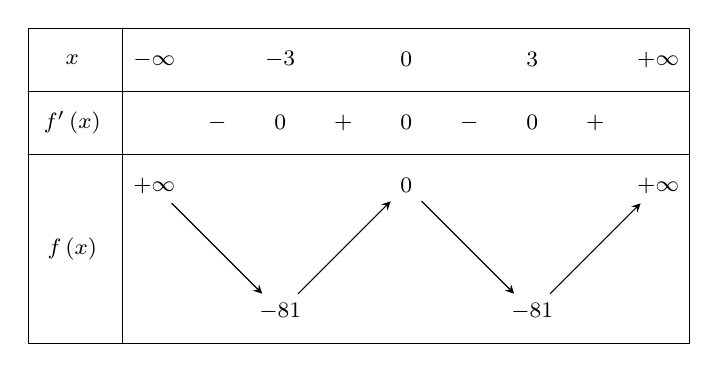
\begin{tikzpicture}[line join = round, line cap = round,font=\footnotesize,>=stealth,scale=.8]
				\foreach \x/\g in{-.3/x,1/-\infty,3/-3,5/0,7/3,9/+\infty}\path(\x,0)node{$\g$};
				\foreach \x/\g in {-.3/f'\left(x\right),2/-,3/0,4/+,5/0,6/-,7/0,8/+}\path(\x,-1)node{$\g$};
				\foreach \x/\y/\g in {-.3/-3/f\left(x\right),1/-2/+\infty,3/-4/-81,5/-2/0,7/-4/-81,9/-2/+\infty}\path(\x,\y)node(\x){$\g$};
				\foreach \x/\y in {1/3,3/5,5/7,7/9}\draw[-stealth] (\x)--(\y);
				\draw (-1,.5) rectangle (9.5,-4.5)
				(-1,-.5)--(9.5,-.5)
				(-1,-1.5)--(9.5,-1.5)
				(.5,.5)--(.5,-4.5);
				\end{tikzpicture}
			\end{center}
			Để hàm số $y=f\left(x^4-18 x^2+m\right)$ có đúng $7$ cực trị thì $y=f'\left(x^4-18 x^2+m\right)=0$ có $4$ nghiệm bội lẻ phân biệt khác $0$ và  khác $\pm 3$ thì
			$$
			\Leftrightarrow\hoac{& - 8 1 < - m + 8 2 < 0  \\&	- m \geq 0 } \Leftrightarrow \hoac{&	82<m<163 \\&m \leq 0 \, \text{(loại)}.}$$
			Vì $m \in \mathbb{N}^*$ nên $m \in\{83,84, \ldots \ldots, 161,162\}$ nên có $80$ giá trị $m$ thỏa yêu cầu bài toán.
		\end{itemize}
	}
\end{ex}

\Closesolutionfile{ans}
\indapan{6}{ans/ans-2-OTC1-TLN}